\section*{1. Nichos de mercado}

\subsection*{Docker}
Docker se posiciona principalmente en el nicho de mercado de desarrolladores de software, empresas tecnológicas y proveedores de servicios en la nube que buscan una solución para la creación, implementación y gestión de aplicaciones en contenedores \citep{Hill2025}. Su capacidad de automatizar despliegues y garantizar la portabilidad entre entornos lo convierte en una opción ideal para DevOps y desarrollo ágil \citep{Mag2025}.

\subsection*{Podman}
Podman está orientado a entornos empresariales y desarrolladores que requieren una solución de contenerización sin \textit{daemon}, compatible con OCI y con enfoque en la seguridad \citep{Surendhar2024}. Su naturaleza sin \textit{daemon} y su capacidad para ejecutar contenedores de forma aislada permiten su adopción en entornos donde la seguridad y la conformidad son prioridades \citep{Trevor2022}.

\subsection*{Udocker}
Udocker se especializa en nichos de mercado académicos y de investigación, donde los usuarios necesitan ejecutar contenedores sin privilegios en sistemas que no permiten la instalación de software de nivel de sistema \citep{Campos2017}. Su facilidad para funcionar en entornos HPC (Computación de Alto Rendimiento) sin requerir permisos de root lo hace adecuado para instituciones de investigación \citep{Gomes2018}.

\subsection*{Wasm (WebAssembly)}
Wasm se centra en el nicho de desarrollo web y aplicaciones de alto rendimiento en el navegador \citep{Haas2017}. Su capacidad para ejecutar código de forma eficiente en múltiples plataformas, incluidas aplicaciones de escritorio y móviles, lo convierte en una opción atractiva para empresas de desarrollo de software que buscan optimización multiplataforma \citep{Jangda2019}.

\subsection*{LXC (Linux Containers)}
LXC es popular en entornos de virtualización ligera y servidores, donde se requiere un control granular sobre los entornos de contenedores \citep{Silva2024}. Su uso está orientado a proveedores de alojamiento web, desarrolladores de software y administradores de sistemas que necesitan un control preciso del entorno del sistema operativo \citep{Simon2023}.

\subsection*{Containerd}
Containerd está dirigido a proveedores de servicios en la nube y plataformas de orquestación como Kubernetes, donde se requiere una solución de gestión de contenedores ligera y compatible con OCI \citep{Vano2023}. Su arquitectura modular lo convierte en una opción preferida para grandes infraestructuras \citep{Zhou2021}.

\subsection*{LXD}
LXD se enfoca en nichos de mercado que requieren entornos de virtualización basados en contenedores que imiten máquinas virtuales, como proveedores de servicios en la nube, plataformas de pruebas y entornos de desarrollo \citep{Silva2024}. Su capacidad para ofrecer entornos de sistema completo lo hace ideal para desarrolladores y administradores de sistemas \citep{Kaiser2022}.

\subsection*{Rkt}
Rkt fue diseñado para satisfacer las necesidades de proveedores de servicios en la nube y organizaciones que buscan una alternativa a Docker con un enfoque en la seguridad y compatibilidad OCI \citep{Lingayat2018}. Aunque su desarrollo ha sido discontinuado, sigue siendo relevante en entornos donde la compatibilidad y la seguridad son críticas \citep{Watada2019}.

\subsection*{Singularity}
Singularity se centra en entornos de computación científica y HPC, donde se requiere portabilidad de aplicaciones sin necesidad de privilegios de root \citep{10.1145/3332186.3332192}. Es ampliamente adoptado en universidades, centros de investigación y laboratorios que ejecutan aplicaciones de alto rendimiento \citep{Kurtzer2017}.

\subsection*{runC}
runC está orientado a proveedores de servicios en la nube, plataformas de orquestación como Kubernetes y desarrolladores de software que buscan una solución de contenedorización ligera y compatible con OCI \citep{Perez2005}. Su adopción en proyectos de gran escala se debe a su eficiencia y cumplimiento de estándares de contenedores \citep{151962df5f7e4b9faba0629540c11439}.

\subsection*{CRI-O}
CRI-O está diseñado específicamente para su integración con Kubernetes, sirviendo como un motor de contenedores ligero y compatible con OCI para esta plataforma \citep{CNCF2019}. Es una solución ideal para proveedores de servicios en la nube y organizaciones que utilizan Kubernetes como su plataforma de orquestación principal \citep{151962df5f7e4b9faba0629540c11439}.

\subsection*{Hyper-V Containers}
Hyper-V Containers están orientados a empresas que utilizan infraestructuras basadas en Windows, ofreciendo una solución de contenedorización segura y eficiente para aplicaciones basadas en Windows \citep{Smith2016}. Su integración con el ecosistema de Microsoft lo hace ideal para empresas con infraestructuras híbridas \citep{Clark2024}.

\subsection*{OpenVZ}
OpenVZ se centra en proveedores de alojamiento web y servicios VPS, donde se requiere una solución de virtualización ligera basada en contenedores que permita un control granular sobre los recursos del sistema y la administración de múltiples instancias \citep{OpenVZ2015}.

\subsection*{Linux VServer}
Linux VServer está orientado a administradores de sistemas y proveedores de servicios que requieren una solución de virtualización ligera basada en contenedores para la administración de servidores seguros y eficientes \citep{10.1145/1272996.1273025}. Es una opción adecuada para entornos de servidor dedicados y alojamientos compartidos \citep{LinuxVirt2017}.

\subsection*{Google gVisor}
Google gVisor está dirigido a proveedores de servicios en la nube y organizaciones que priorizan la seguridad en sus entornos de contenedores \citep{LopezFalcon2024}. Su arquitectura de \textit{sandbox} proporciona un aislamiento fuerte, lo que lo convierte en una opción atractiva para aplicaciones sensibles \citep{gvisor2025}.

\subsection*{Kata Containers}
Kata Containers se centra en entornos donde se requiere un alto nivel de seguridad y aislamiento, como proveedores de servicios en la nube y empresas que manejan información confidencial \citep{Viktorsson2020}. Su capacidad para combinar la eficiencia de los contenedores con el aislamiento de máquinas virtuales es su principal ventaja \citep{10.1145/1272996.1273025}.

\subsection*{Firecracker}
Firecracker está orientado a proveedores de servicios en la nube y plataformas de cómputo en la nube que requieren micro VMs eficientes y seguras \citep{Jain}. Es una solución ideal para plataformas \textit{serverless} y entornos multi-tenant \citep{246288}.

\subsection*{Sarus}
Sarus está dirigido a entornos de HPC y computación científica, donde los usuarios necesitan ejecutar contenedores de forma segura en sistemas de alto rendimiento \citep{Sarus2021}. Su compatibilidad con estándares de contenedores y su enfoque en la seguridad lo hacen ideal para centros de investigación y universidades \citep{B2020}.

\begin{table}[htbp]
\centering
\rowcolors{2}{gray!10}{white}
\begin{tabularx}{\textwidth}{>{\raggedright\arraybackslash}X 
                                  >{\raggedright\arraybackslash}X 
                                  >{\raggedright\arraybackslash}X 
                                  >{\raggedright\arraybackslash}X}
\rowcolor{gray!30}
\textbf{Tecnologías} & \textbf{Licencias} & \textbf{Términos de uso} & \textbf{Costo} \\

Docker & Apache 2.0 (permisiva) & \href{https://www.docker.com/legal/docker-terms-service/}{link} & Desde los 11 a 24 dólares \\
Podman & Apache 2.0 (permisiva) & \href{https://github.com/containers/podman/blob/main/LICENSE}{link} & Gratis \\
Udocker & Apache 2.0 (permisiva) & \href{https://github.com/indigo-dc/udocker/blob/master/LICENSE}{link} & Gratis \\
Wasm & Apache 2.0 (permisiva) & \href{https://github.com/WebAssembly/design/blob/main/LICENSE}{link} & Gratis \\
LXC & GNU LGPLv2.1+ & \href{https://linuxcontainers.org/lxc/introduction/}{link} & Gratis \\
Containerd & Apache 2.0 (permisiva) & \href{https://github.com/containerd/containerd/blob/main/LICENSE}{link} & Gratis \\
LXD & AGPL-3.0 license & \href{https://github.com/canonical/lxd}{link} & Gratis \\
Rkt & Apache 2.0 (permisiva) & \href{https://github.com/rkt/rkt/blob/master/LICENSE}{link} & Descontinuado \\
Singularity & BSD 3-Clause (permisiva) & \href{https://github.com/sylabs/singularity/blob/main/LICENSE.md}{link} & Singularity CE (Gratis), PRO (\$30/año) \\
runC & Apache 2.0 (permisiva) & \href{https://github.com/opencontainers/runc/blob/main/LICENSE}{link} & Gratis \\
CRI-O & Apache 2.0 (permisiva) & \href{https://github.com/cri-o/cri-o/blob/main/LICENSE}{link} & Gratis \\
Hyper-V containers & Licencia Windows (Propietaria) & \href{https://learn.microsoft.com/es-es/virtualization/windowscontainers/images-eula}{link} & Windows Server 2025 (\$1,176 USD) \\
OpenVZ & GPL v2 (permisiva) & \href{https://openvz.org/}{link} & Gratis \\
Linux VServer & GPL v2 (permisiva) & \href{http://linux-vserver.org/}{link} & Gratis \\
Google gVisor & Apache 2.0 (permisiva) & \href{https://github.com/google/gvisor}{link} & Gratis \\
Kata Containers & Apache 2.0 (permisiva) & \href{https://github.com/kata-containers/kata-containers/blob/main/LICENSE}{link} & Gratis \\
Firecracker & Apache 2.0 (permisiva) & \href{https://github.com/firecracker-microvm/firecracker}{link} & Gratis \\
Sarus & BSD 3-Clause (permisiva) & \href{https://github.com/eth-cscs/sarus}{link} & Gratis \\

\end{tabularx}
\caption{Comparativa de tecnologías de contenerización, licencias, términos de uso y costos}
\end{table}

 \begin{table}[H]
\centering
\scriptsize
\setlength{\tabcolsep}{3pt}
\renewcommand{\arraystretch}{1.1}
\begin{tabularx}{\textwidth}{|p{0.2\textwidth}|p{0.75\textwidth}|}
\hline
\textbf{Tecnología} & \textbf{Interfaz de Uso} \\
\hline
Docker & \CLI\ principalmente, con Docker Desktop para interfaz gráfica. \\
\hline
Podman & \CLI\ similar a Docker, sin daemon. Opcional Podman Desktop. \\
\hline
Udocker & \CLI\ específica para ejecutar contenedores sin privilegios root. \\
\hline
Wasm (WebAssembly) & Ejecución través de navegadores web, \API\ de JavaScript. \\
\hline
LXC & \CLI\ mediante comando lxc, sin interfaz gráfica oficial. \\
\hline
Containerd & \CLI\ con herramientas como ctr, backend para otras herramientas. \\
\hline
LXD & \CLI\ mediante lxd/lxc, con interfaz web LXD Web \UI\ . \\
\hline
Rkt & \CLI\ mediante comandos como rkt run (descontinuado). \\
\hline
Singularity & \CLI\ mediante comandos singularity para gestión de contenedores. \\
\hline
runC & \CLI\ mediante comandos runc, runtime bajo Docker y Kubernetes. \\
\hline
CRI-O & \CLI\, interactúa con Kubernetes, sin interfaz gráfica dedicada. \\
\hline
Hyper-V containers & \CLI\ (PowerShell) o Hyper-V Manager para VMs. \\
\hline
OpenVZ & \CLI\ mediante comandos vzctl, con interfaces gráficas de terceros. \\
\hline
Linux VServer & \CLI\ mediante comandos vserver para gestión. \\
\hline
Google gVisor & \CLI\ mediante comandos estándar de Docker con seguridad adicional. \\
\hline
Kata Containers & \CLI\ mediante kata-runtime, integración con Kubernetes. \\
\hline
Firecracker & \CLI\ mediante API RESTful y herramientas firecracker. \\
\hline
Sarus & \CLI\ mediante comando sarus para entornos \HPC\ . \\
\hline
\end{tabularx}
\caption{Interfaz de uso de cada VBC}\label{tab:interfaz-vbc}
\end{table}
\begin{table}[H]
    \centering
    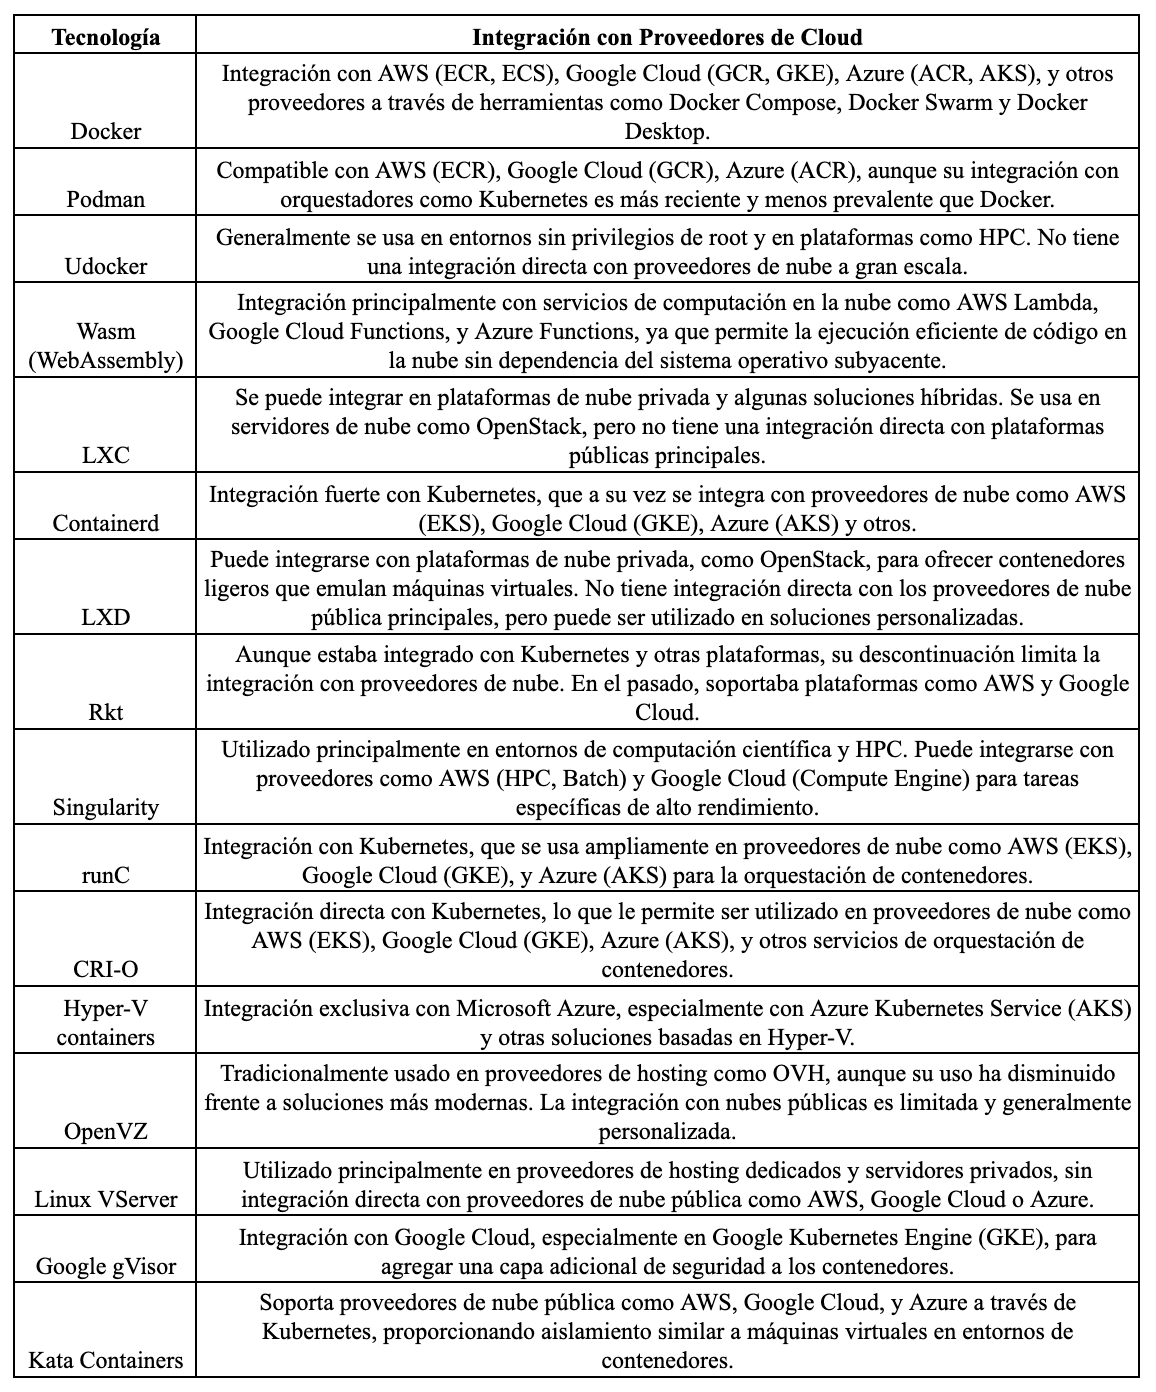
\includegraphics[width=\textwidth] {tablas-images/cp3/integracion-cloud.png}
    \caption{Integración cloud de cada VBC}\label{tab:tabla-integracion-cloud}
\end{table}